\documentclass[11pt]{article}
\setlength{\oddsidemargin}{0in}
\setlength{\evensidemargin}{0in}
\setlength{\textwidth}{6.5in}

\usepackage{fancyhdr}
\pagestyle{fancy}
\usepackage{amsmath,amsfonts,amssymb}
\usepackage{epsfig}
\usepackage{subfigure}
\usepackage{placeins}
\usepackage{amsmath}
\usepackage[usenames,dvipsnames,svgnames,table]{xcolor}
\usepackage{amssymb}
\usepackage{setspace}
\usepackage{graphicx} % Include figure files
\usepackage{times}
\usepackage{amsthm}
\usepackage{hyperref}
\usepackage{enumitem}
\hypersetup{bookmarks=true, unicode=false, pdftoolbar=true, pdfmenubar=true, pdffitwindow=false, pdfstartview={FitH}, pdfcreator={Daniel Larremore}, pdfproducer={Daniel Larremore}, pdfkeywords={} {} {}, pdfnewwindow=true, colorlinks=true, linkcolor=blue, citecolor=Green, filecolor=magenta, urlcolor=cyan,}
\usepackage[parfill]{parskip}

% styling for solution blocks
\newenvironment{solution}{\par\noindent\begingroup\color{BrickRed}\textbf{Solution:} }{\par\endgroup}

% This little bit tells LaTeX where to look for figures.
% As written, it says to look first in Notes/figs_python, and then look in the current directory ./  
\graphicspath{{../Notes/figs_python/}{./}}

\begin{document}

\lhead{{\bf Mathematical \& Computational Modeling of Infectious Diseases \\ 
Homework 1}}
\rhead{{\bf Jason Hunter\\2025}}
\renewcommand{\headrulewidth}{0.4pt}

{\bf Instructions:} 
\begin{itemize}[itemsep=-7pt]
	\item Please turn in a single PDF file.
	\item Please share a link to your code, but do not attach the actual code. 
	\item Don't forget to list anyone you collaborated with. 
\end{itemize}
\vspace{0.1in}\hrule

\begin{enumerate}

\item The goal of this problem is to get you over any barriers with 
	  (i) getting Python set up, 
	  (ii) getting the SIR model implemented in a Forward Euler solver, and
	  (iii) getting matplotlib set up.

Write a function in Python that uses the Forward Euler method to simulate the SIR model {\it
in which the population is slowly growing}.
In your simulations, suppose that we have an initial population of size $N=1000$, with $I_0=1$, $S_0=999$.
Suppose that
$\beta=1$, $\gamma=0.5$,
and then
$\mu_{\text{birth}}=0.01$
and
$\mu_{\text{death}} = \tfrac{1}{2} \mu_\text{birth}$.


Produce a single plot that captures the dynamics of transmission over the appropriate amount of time
for the population to grow by 50\% to a total of $N=1500$.
Be sure to include a legend and your name in the title of the plot.

% image scaled to fit on the current page
\begin{center}
  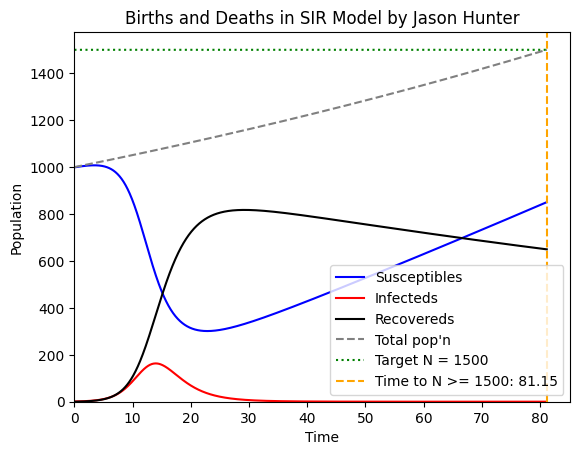
\includegraphics[width=0.9\textwidth, height=0.6\textheight, keepaspectratio]{births-and-deaths.png}
\end{center}

\clearpage

\item The goal of this problem is to show an important fact about transition rates in compartmental models.
	  It is also a good chance to become refreshed on simple ODE solving and separation of variables.
	  Finally, it makes good on a promise made in lecture notes to ask this homework question!
	  Imagine that we are interested in SIR dynamics,
	  but everyone starts out either infected or recovered,
	  and no one starts out susceptible.
\begin{enumerate}[label=\alph*.]
	\item Use this information to simplify the typical equation for $\dot{I}$.
		\begin{solution} \newline
		If no one is susceptible, I can effectively set $S=0$ in the equation for $\dot{I}$.
		The original equation for $\dot{I}$ is: 
		$$\dot{I} = \beta S I - \gamma I$$
		Simplifiying with $S=0$ gives:
			\begin{align*}
			\dot{I} &= \beta (0) I - \gamma I \\
			\dot{I} &= - \gamma I
			\end{align*}
		\end{solution}

	\item Solve your simplified differential equation with the initial condition $I(0) = I_0$.
		\begin{solution} \newline
			Given:
			$$\dfrac{dI}{dt} = -\gamma I$$
			First I do some dividing out of $I$ and some multiplying by $dt$:
			$$\dfrac{dI}{I} = -\gamma dt$$
			Then I integrate both sides:
			\begin{align*}
			\int \dfrac{dI}{I} &= \int -\gamma dt \\
			\ln|I| &= -\gamma t + C
			\end{align*}
			Then I do some magic tricks via exponentiating both sides:
			$$I = e^{-\gamma t + C} = e^C e^{-\gamma t}$$
			And finally, letting $e^C = I_0$ (the initial condition $I(0) = I_0$):
			$$I(t) = I_0 e^{-\gamma t}$$
		\end{solution}

	\item Manipulate your solution to derive the fraction of the initially infected people who are still infected at time $t$.
		\begin{solution} \newline \newline
			To find the fraction of initially infected people who are still infected at time $t$,
			All I need to do is divide $I(t)$ by $I_0$:
			$$\frac{I(t)}{I_0} = \frac{I_0 e^{-\gamma t}}{I_0} = e^{-\gamma t}$$
			So at a given time $t$, the fraction still infected is $e^{-\gamma t}$.
		\end{solution}

	\item Discuss this equation. 
		  What does it do over time?
		  How is it related to the fraction of infected people who have {\it left} the infected class?
		\begin{solution} \newline \newline
			\textit{What does it do over time?} \\ \\
				The equation $e^{-\gamma t}$ is essentially just exponential decay. \\
				As time $t$ increases, the whole term $e^{-\gamma t}$ decreases/trends towards $0$. \\
				In other words, the epidemic is dying out over time. \\ \\
			\textit{How is it related to the fraction of infected people who have left the infected class?} \\ \\
				It is the complement to the fraction of initially infected people who have left the I class.
		\end{solution}
			
	\item This formula produces values between 0 and 1,
		  and it tells us the probability that a randomly chosen infected person is still infected at time $t$.
		  How does this relate to the cumulative distribution function (CDF) 
		  that describes the probability that someone is infected for less than or equal to $t$ units of time? 
		  Take a derivative of the CDF to get a PDF for the duration of infection lengths is. 
		  Then, find out what this famous probability distribution is called, and write down its expected value.
		\begin{solution} \newline \newline
			Given that the formula $e^{-\gamma t}$ is representative of the probability that a randomly chosen infected person is still infected at time t.
			The CDF, which describes the probability that someone is infected for less than or equal to $t$ units of time, is the complement of this formula:
			$$F(t) = 1 - e^{-\gamma t}$$
			Taking the derivative of the CDF to get the PDF:
			\begin{align*}
			f(t) &= \dfrac{d}{dt} F(t) \\
				 &= \dfrac{d}{dt} (1 - e^{-\gamma t}) \\
			f(t) &= \gamma e^{-\gamma t}
			\end{align*}
			This is the exponential distribution. \\
			By definition:
			$$E[X] = \int_0^\infty t f(t) dt$$
			So plugging in our PDF:
			$$E[X] = \int_0^\infty t \gamma e^{-\gamma t} dt$$
			Using integration by parts, I get:
			$$E[X] = \frac{1}{\gamma}$$
		\end{solution}

	\item Use your results to explain how the recovery rate $\gamma$ is related to the typical amount of time a person remains infectious.
		\begin{solution} \newline \newline
			If $E[X] = \frac{1}{\gamma}$ can be used to model the typical amount of time a person stays infected for,
			then $\gamma$ must be the inverse of the expected duration of infection. \\
			Assuming that time steps are measured in days, \\
			if $\gamma$ is say $2$, then the expected duration of infection is just half of a day. \\
			Conversely, if $\gamma$ is $0.5$, then the expected duration of infection is $2$ whole days. \\
			So the larger the recovery rate $\gamma$, the shorter the expected duration of infection. \\
			This is somewhat intuitive.
		\end{solution}
\end{enumerate}

\clearpage

\item The goal of this problem is to 
	  (i) figure out how to solve the final epidemic size equation, and 
	  (ii) test the equation's predictions.

	\begin{enumerate}[label=\alph*.]
		\item First, explain how an epidemic's total size, also called its cumulative incidence, is related to $s_\infty$ and $r_\infty$. 
			\begin{solution} \newline \newline
				I'm going to finish this tomorrow with the group. \\
			\end{solution}
		\item Recall that 
		\begin{equation}r_\infty = 1-e^{-R_0 r_\infty}\label{myeq}\end{equation} 
		Though we can't solve this equation, we can use a valuable graphical technique as follows. 
		First, we define a function $f(r_\infty) = r_\infty$ and define a second function $g(r_\infty) = 1-e^{-R_0 r_\infty}$. 
		Note that $f$ is the left hand side of Eq.~\eqref{myeq}, while $g$ is the right hand side. 
		This allows us to plot $f$ and plot $g$, both as a function of $r_\infty$, to see where they cross---that is, where $f=g$. 
		
		Create four plots for $R_0 \in \{0.9, 1.0, 1.1, 1.2\}$ with $f$ in black and $g$ in red. 
		Use the {\bf fsolve} function to find the intersection point, and use matplotlib's {\bf scatter} function to plot a blue circle at the intersection. \footnote{Hint, use \href{https://docs.scipy.org/doc/scipy/reference/generated/scipy.optimize.fsolve.html}{the fsolve docs}, 
		and note that, because fsolve wants to find roots (points where a function is zero), 
		you can create an auxiliary function $h(r_\infty) = f(r_\infty)-g(r_\infty)$ 
		which will be equal to zero at the point where $f$ and $g$ intersect!}
			\begin{solution}
				See my graph on the following page.
			\end{solution}
		\begin{center}
		  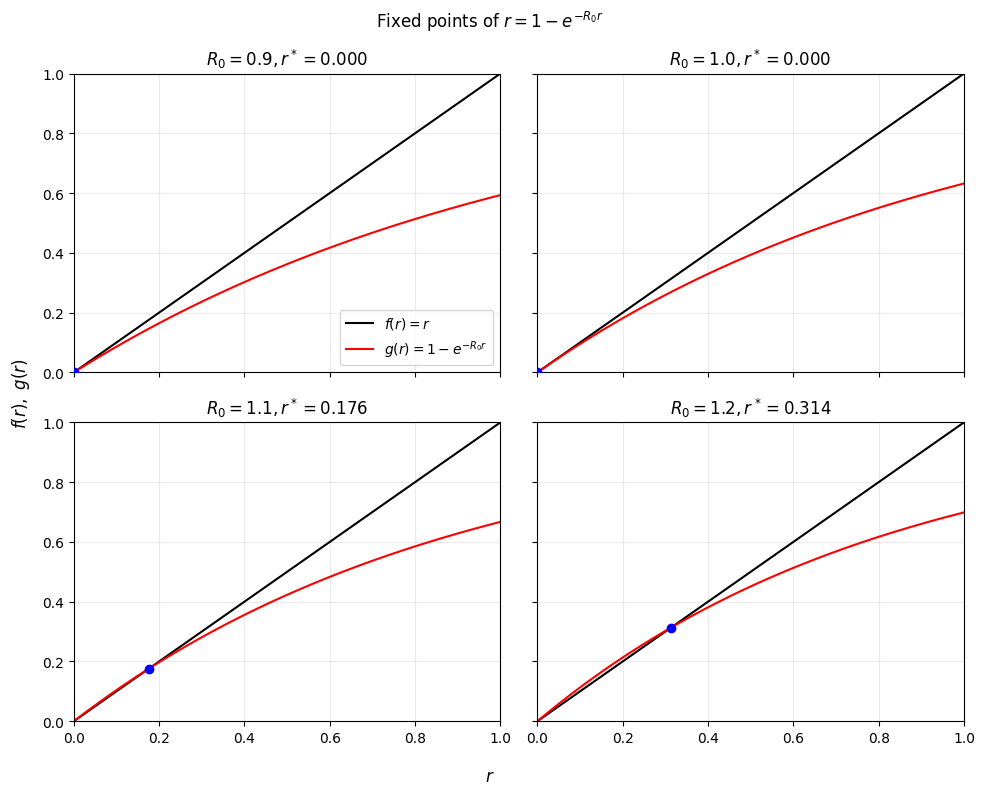
\includegraphics[width=0.9\textwidth, height=0.6\textheight, keepaspectratio]{final_size_plots.png}
		\end{center}

		
		\item Comment on what you see in the plots in the context of what we have learned about $R_0$. 
		      What do you see in your figures? What happens when $R_0 < 1$?
		\item Finally, test the predictions made by this final-size equation by using your SIR code and $\beta=1$, $\gamma=0.5$ by creating a new version of that epidemic with a green dotted line at the height of $r_\infty$. Does this final size prediction work?\footnote{Take care, as the units of our SIR plots and the units of our final size prediction are not the same! You may have to do a conversion...}
	\end{enumerate}
	

\clearpage
\item (Grad / EC): In class, we showed that the SIR model's disease-free equilibrium is stable when $s<\tfrac{1}{R_0}$ and unstable otherwise. 
	  Using $N=10^6$, and $\varepsilon = \frac{1}{N}$ as your perturbation, 
	  produce a single figure {\it using your simulation code and its output} that illustrates this point.
	  Write a caption that explains the principle of stability, and explain how your figure illustrates it.
\footnote{There are many possible ways to make such a figure, and write its caption! 
One could use all of the outputs of the simulation, for instance, 
but one could also use just those that illustrate the intended point.}

\end{enumerate}



\end{document}